\chapter{Experimental Setup}
\label{chapter: experimental setup}

Now that the spectrometer designs and important background information are 
established, I will describe the experimental setup for the laser-only 
experiment of May 2023. The main goals of the experiment are to assess the performance of the 
spectrometers, test backlighter materials, and to validate the setup as a 
whole. As the main focus of this work are the spectrometers, I will only 
schematically explain the general experimental setup in section \ref{section: general setup}, followed by a detailed presentation the mechanical design of the spectrometers in section \ref{section: mechanical design}. 

\section{General Setup}
\label{section: general setup}

The experimental setup, as shown schematically in fig. \ref{fig: setup 
schematic} and as an \textit{Inventor} model in fig. \ref{fig: setup inventor}, 
consists of five main components: the backlighter target, aluminum sample, 
spectrometers, 
PHELIX beam, and focus diagnostics. To note 
is that the location of heavy-ion 
beam is also taken into account by the setup. Laser shots that use an aluminum 
sample are denoted as 
absorption shots, while reference shots without samples are called source 
shots, where the word shot is used interchangeable with event. From each event results one set of 
spectra. In the following, I will describe each component individually.

The backlighter targets are irradiated with the PHELIX laser to form plasmas as 
x-ray sources for the sample diagnostics. The PHELIX pulses last \SI{2}{\nano\second} and have an energy of up to \SI{200}{\joule}. The pulses are focused onto the backlighter targets with a spot size of $\sim30$-\SI{40}{\micro\meter} (FWHM). For part of the shots, a phase plate was inserted into the 
PHELIX beam to smooth the beam by introducing a random, spatially distributed phase. This leads to a larger focus spot of \SI{145}{\micro\meter} in the vertical direction (perpendicular to the breadboard) and \SI{120}{\micro\meter} in the horizontal, as calculated by Alice Renaux \citep{alice_report}. The fine-scale spatial structure in the beam smooths the heating of the backlighter target through thermal conduction \citep{dixit1993random}. Thus the fluctuation between shots was reduced and the plasma conditions were changed. The focus diagnostics consist of an optical setup designed to 
image the TCC onto a camera that lies outside the vacuum chamber and are used to 
align the targets and PHELIX beam under vacuum, as well as focus the latter.

To find an optimal backlighter for 
future experiments, a variety of materials are tested, including the rare 
earths samarium (Sm), gadolinium (Gd), terbium (Tb), dysprosium (Dy), along 
with gold (Au) and polytetrafluoroethylene (PTFE), also known by the brand name Teflon. In 
addition, aluminum (Al) targets are used, 
fulfilling the purpose of characterizing the spectrometers and validating the 
setup using a well-described line emission source. All of the targets are 
rectangular foils with a variety of thicknesses: \SI{100}{\micro\meter} for the 
rare earths, \SI{20}{\micro\meter} for gold, \SI{120}{\micro\meter} for Teflon and \SI{20}{\micro\meter} or 
\SI{50}{\micro\meter} for aluminum. The targets are affixed to holders placed 
on a target ladder and aligned to the target chamber center (TCC) for 
each event. These holders also position the aluminum samples at the 
aforementioned \SI{5}{\milli\meter} away from the backlighters. To note is that targets with and without samples are prepared depending on whether the shot is an absorption or source shot respectively.

The samples are penetrated by the x-rays, which are transmitted to the 
spectrometers. The location of the samples is such that they lie in the optical 
path of the FSSR-1D and the bottom channel (w.r.t fig. \ref{fig: setup 
schematic}) of the DUCC. The samples come in two thicknesses, either
\SI{0.8}{\micro\meter} or \SI{2}{\micro\meter}, and are cold (at ambient temperatures), i.e. have no dedicated heating setup.

The spectrometers then disperse and detect the source and transmitted x-rays. As seen in fig. \ref{fig: setup schematic}, the layout is such that 
during an absorption shot the FSSR-1D and bottom channel of 
the DUCC record transmitted spectra, while the SUCC and upper channel of 
the DUCC take reference, or source, spectra. All spectrometers are fixed in the chamber, but due to the limitation of only 
having two GE-VAC 2048 512 series x-ray cameras from \textit{greateyes}, the cameras are switched between spectrometers depending on the purpose of a shot. Generally speaking, one of the cameras is 
attached to the SUCC, yielding wide energy range reference spectra, while the 
other is on either the DUCC or FSSR-1D. Different filters were placed in front of the spectrometers for protection and to avoid saturation of the camera. Between shots, filters were often 
changed to accommodate different backlighter intensities, which depend on laser 
energy and backlighter material. In total, four filter materials were used: 
carbon, gold, pokalon, and polycarbonate. All the spectrometers are orientated so that they view the 
backlighter at the same radial angle, exploiting the assumed conical symmetry 
of the plasma emissions. As such, the SUCC is tilted upwards and positioned 
above the upper DUCC channel, along with the view of the FSSR-1D placed 
slightly above the lower channel of the DUCC. Consequently, only the FSSR-1D 
lies in the plane containing the PHELIX beam and parallel to the breadboard at the chamber floor. If the OSUCC is used, it replaces the FSSR-1D in the experimental scheme, and accordingly is placed such that it can be used for transmitted spectra.

\begin{figure}[H]
	\centering
	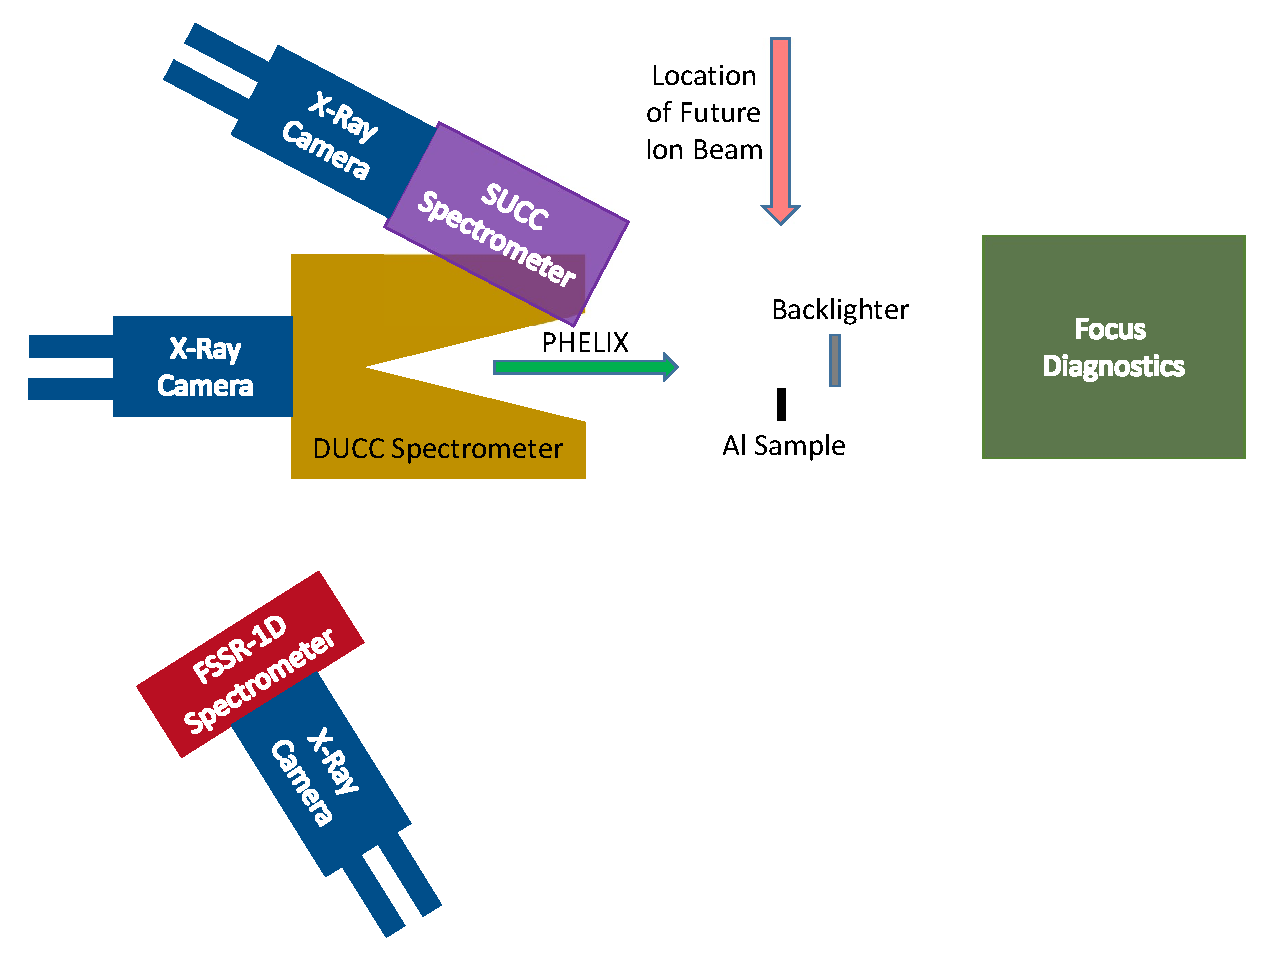
\includegraphics[width = 0.79\textwidth]{Diagrams/Experimental_setup_schematic.pdf}
	\caption{Schematic illustration of the experimental setup. Note that the 
	location of the heavy-ion beam for future experiments is marked, but of 
	course not present in this experiment. The DUCC and SUCC spectrometers are 
	not in the plane of the illustration, but tilted downwards and upwards 
	respectively. At any one time there are only two cameras in the setup. The x-ray cameras can be freely transferred between the 
	spectrometers.}
	\label{fig: setup schematic}
\end{figure}

\begin{figure}[H]
	\centering
	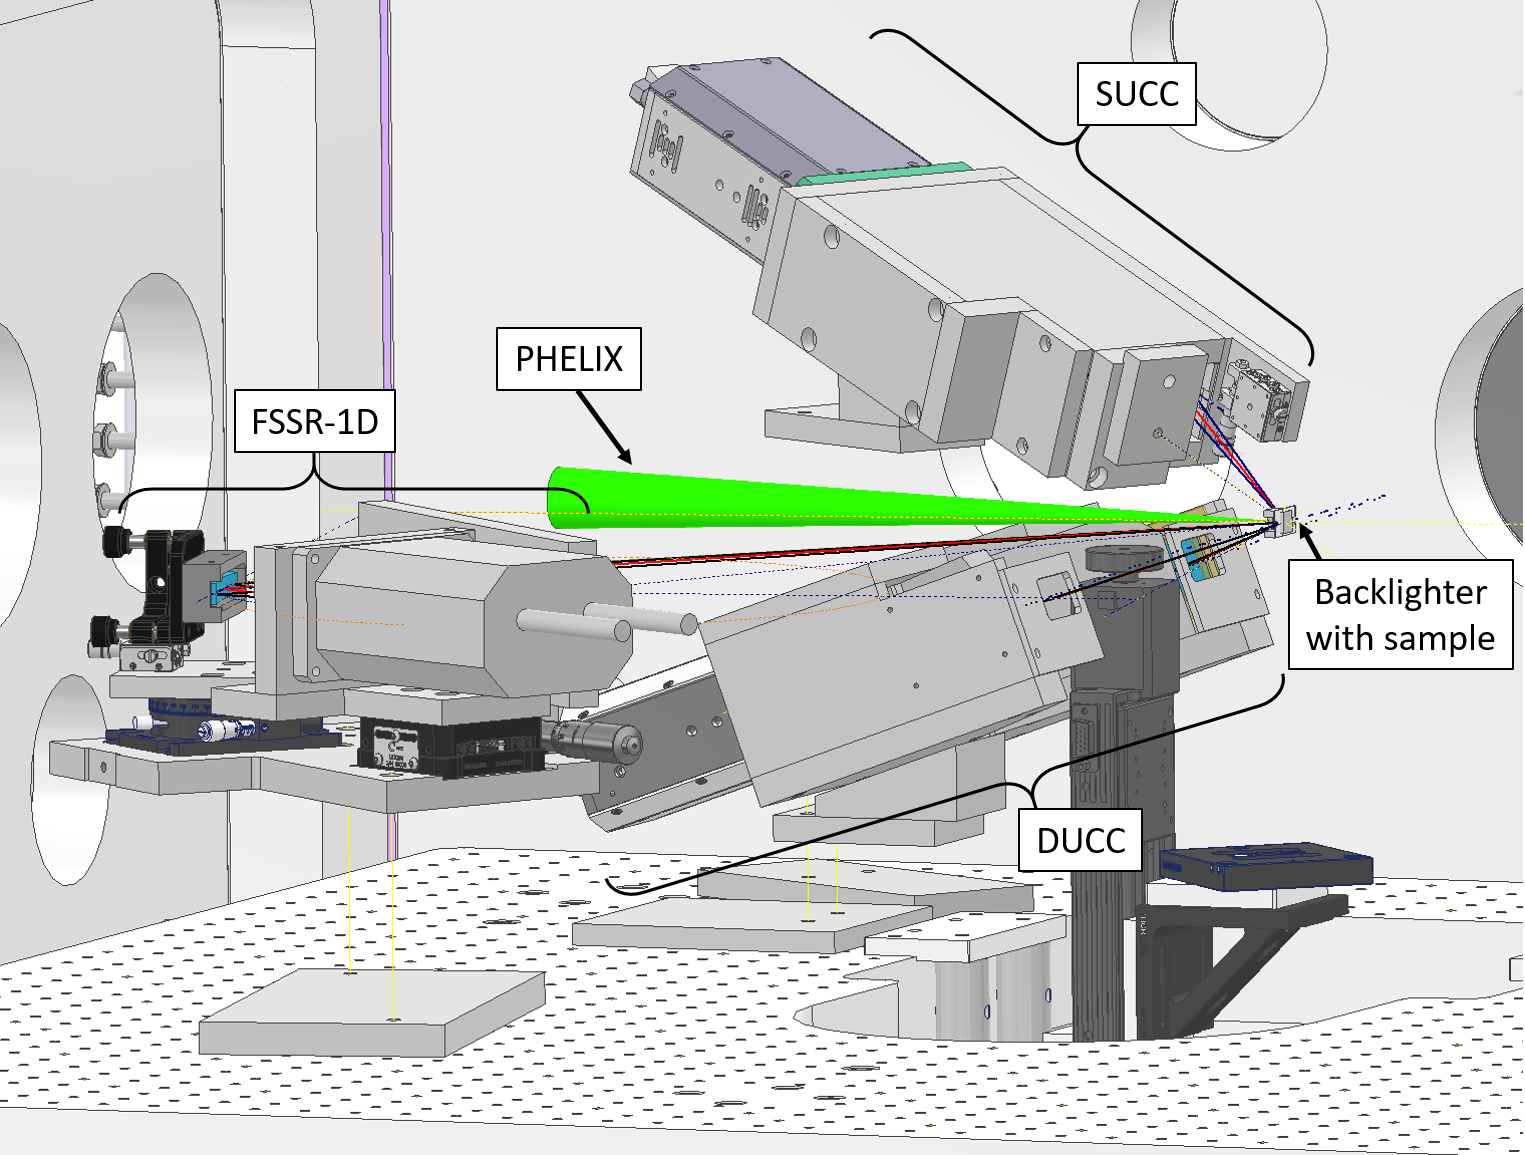
\includegraphics[width = 0.7\textwidth]{Diagrams/Inv_HHT_labeled.PNG}
	\caption{\textit{Inventor} model of the HHT chamber from the perspective of 
	the 
	bottom right of fig. \ref{fig: setup schematic} looking towards the 
	spectrometers. The heavy-ion beam as well as the focus diagnostics are not 
	pictured. The optical posts that connect the spectrometers to their bases 
	are not shown, but their locations are depicted with thin yellow lines. 
	Additionally, the optical paths in the dispersive direction for each 
	spectrometer are shown in blue, with a red line for the central rays. In 
	actuality the PHELIX beam extends out of the chamber.}
	\label{fig: setup inventor}
\end{figure}

\section{Mechanical Design of Spectrometers}
\label{section: mechanical design}

I based the mechanical design of the spectrometers around four goals. First, 
the devices must implement the designs presented in chapter \ref{chapter: 
spectrometer design} to an approximately $\pm$\SI{0.5}{\milli\meter} precision, 
ensuring that sufficient internal and external alignment to produce 
well-resolved spectra is achieved. Second, the crystal and camera chip must be 
sufficiently shielded while still maintaining enough intensity on the detector. 
Third, alignment of the spectrometer components to one another and the 
backlighter must be addressed. This requirement is more stringent for the 
FSSR-1D as a consequence of its focusing properties. Finally, the devices must 
be robust enough to withstand the harsh experimental conditions resulting from 
the heavy-ion beam and plasma. This mainly takes the form of heavy aluminum 
shielding, among others.

In this section, I will describe the 
mechanical designs of the DUCC and FSSR-1D, whose models are built in the CAD 
program \textit{Autodesk Inventor 2020}. The SUCC will not be elaborated on, as 
it is not designed by me and generally shares a similar mechanical design 
philosophy with a single channel of the DUCC. All spectrometers are 
outfitted with in-vacuum 
CCD cameras from \textit{greateyes} of the GE-VAC 2048 512 
series as detectors. In the case of the DUCC, an adjusted camera 
with a thinner front plate is used to avoid clipping. The 
spectrometer parts are generally made of aluminum, unless otherwise 
specified.


\subsection{Dual Unbent Crystal Spectrometer}

The DUCC model is shown in fig. \ref{InvDUCC} with the parts 
color 
coded, which is presented in table \ref{Table: DUCC colors}, 
along with 
a summary of their functions and names. The 
most numerous parts are the ones responsible for shielding and 
structure. These protect the chip and crystals from debris, 
particles 
and extraneous rays. Also serving a shielding role is a pointer 
holder, 
whose main purpose is to hold the optical post for alignment 
purposes.

\begin{table}[H]
	\centering
	\caption{Color code of the DUCC model with the functions and name 
		of 
		the parts.}
	\vspace{0.05cm}
	\renewcommand{\arraystretch}{1.5}
	\centering
	\begin{tabular}{|c|c|c|} 
		\hline
		Color & Function & Name \\ [0.5ex]
		\hline\hline
		Light gray & Structural/Shielding & - \\ 
		[0.5ex]
		\hline
		White (near source) & Protecting crystal & Blast shield \\ 
		[0.5ex]
		\hline
		White (labeled) & Capturing spectra & Greateyes camera\\ 
		[0.5ex]
		\hline
		Brown & Capturing spectra & Camera chip \\ 
		[0.5ex]
		\hline
		Dark gray & Holding alignment post & Pointer holder \\ 
		[0.5ex]
		\hline
		Red (front of camera) & Separating spectra/holding filter & 
		Filter holder \\ [0.5ex]
		\hline
		Transparent yellow & Securing crystals & Crystal frame \\ 
		[0.5ex]
		\hline
		Turquoise & Dispersion of rays & ADP crystal \\ [0.5ex]
		\hline
		Green & Supporting + tilting spectrometer & Foot with angled 
		block \\ 
		[0.5ex]
		\hline
		Beige & Display location of chamber floor & Breadboard floor \\ 
		[0.5ex]
		\hline
		Red & - & Central ray \\ 
		[0.5ex]
		\hline
		Black & - & Outer rays \\ [0.5ex]
		\hline
	\end{tabular}
	\label{Table: DUCC colors}
\end{table}

The blast shields, on which \SI{2}{\micro\meter} Mylar foils are 
attached to the opening, protect the crystal from debris while 
allowing 
the x-rays through. Additionally, two carbon filters are glued 
onto the 
openings of the filter holder, which are light-tight and prevent 
visible light from reaching the chip. These carbon 
filters can be chosen to have an areal density of 
$\approx\SI{200}{\micro\gram\per\cm\squared}$ or 
$\approx\SI{900}{\micro\gram\per\cm\squared}$, depending on the 
intensities observed on the chips in the experiment. The filter 
holder 
also 
serves to spatially separate the two channels 
onto the chip, where the holes have a vertical separation of 
\SI{1}{\milli\meter} so that a shadow will appear on the center 
line of 
the chip.

The ADP crystals are held in place by first placing them in a 
groove, 
then screwing on the crystal frames made of Trovidur. By 
attaching a 
plexiglass foil to the bottom of the groove and fabricating the 
frames 
out of plastic, the crystal is protected from direct contact with 
the 
aluminum housing. The $20\degree$ angle of the DUCC w.r.t. the 
PHELIX 
beam is implemented by an angled block of the foot. Finally, a 
venting 
channel is engraved into the plate attached to the camera, 
partially 
visible in fig. \ref{InvDUCCFullBack}. This channel is designed 
with 
random turns, similar to a snake, so that air can escape while 
light is 
kept out. This is essential to prevent the carbon filters from 
breaking 
during venting of the HHT chamber.


The alignment is realized by first affixing the pointer holder 
with 
screws to 
the top and bottom plates of the shielding, making sure to use 
the 
groove on 
the bottom plate to guarantee proper orientation. Then an optical 
post 
is set 
to the designed distance from the front surface of the pointer 
holder 
to the 
x-ray source. The post is attached to the pointer holder and the 
DUCC 
is brought into 
the chamber. Once the tip of the post is as close as possible to 
the 
laser-target interaction point, known as the target chamber 
center 
(TCC), the spectrometer is aligned, as the alignment of 
further degrees of freedom
is guaranteed by the mechanical precision of the structural 
pieces, reaching the desired precision of $\pm$\SI{0.5}{\milli\meter}.

\begin{figure} [H]
	\centering
	\begin{subfigure}[t]{0.34\textwidth}
		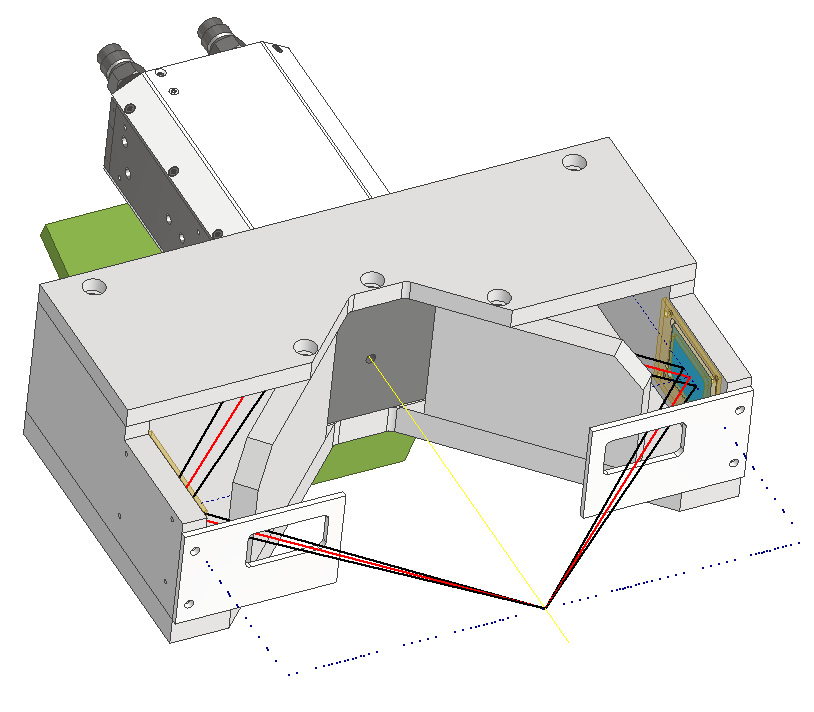
\includegraphics[width=\textwidth]{InventorPics/FullDUCC.PNG}
		\caption{Front view.}
		\label{InvDUCCFullFront}
	\end{subfigure}%
	\hfill
	\begin{subfigure}[t]{0.64\textwidth}
	\centering
		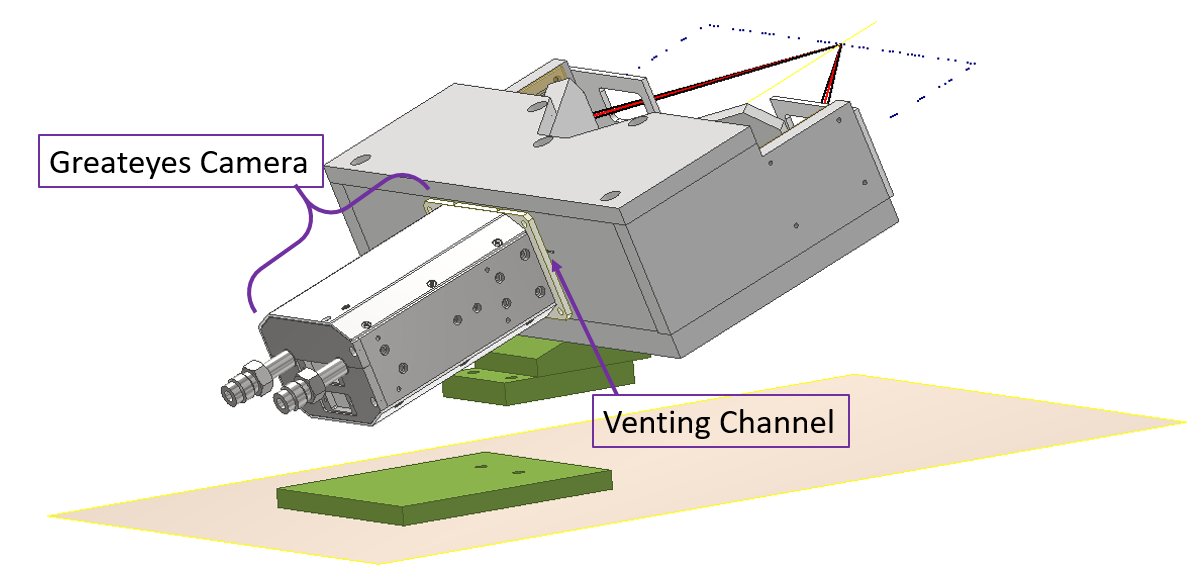
\includegraphics[width=\textwidth]{InventorPics/FullDUCCBack.PNG}
		\caption{Back view with Greateyes camera and venting 
		channel 
		labeled.}
		\label{InvDUCCFullBack}
	\end{subfigure}\\[1ex]
	\centering
	\begin{subfigure}[t]{0.35\textwidth}
		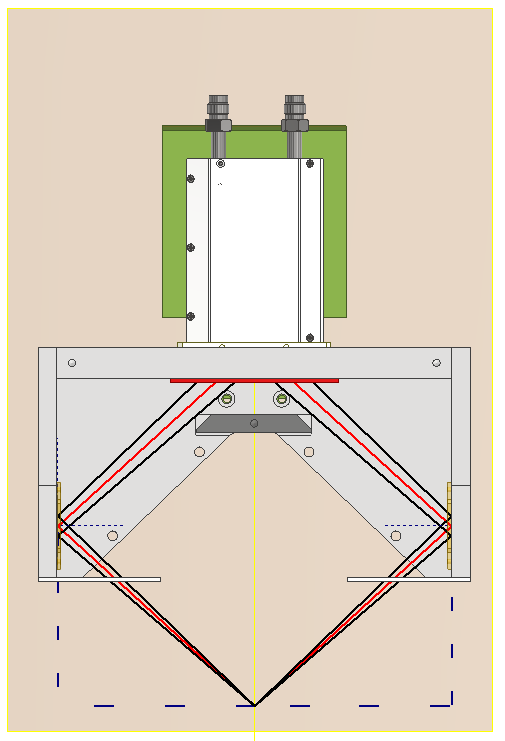
\includegraphics[width=\textwidth]{InventorPics/DUCCTopWoCover.PNG}
		\caption{Top view with top and inner shielding hidden.}
		\label{InvDUCCPartTop}
	\end{subfigure}%
	\hfill
	\begin{subfigure}[t]{0.63\textwidth}
	\centering
		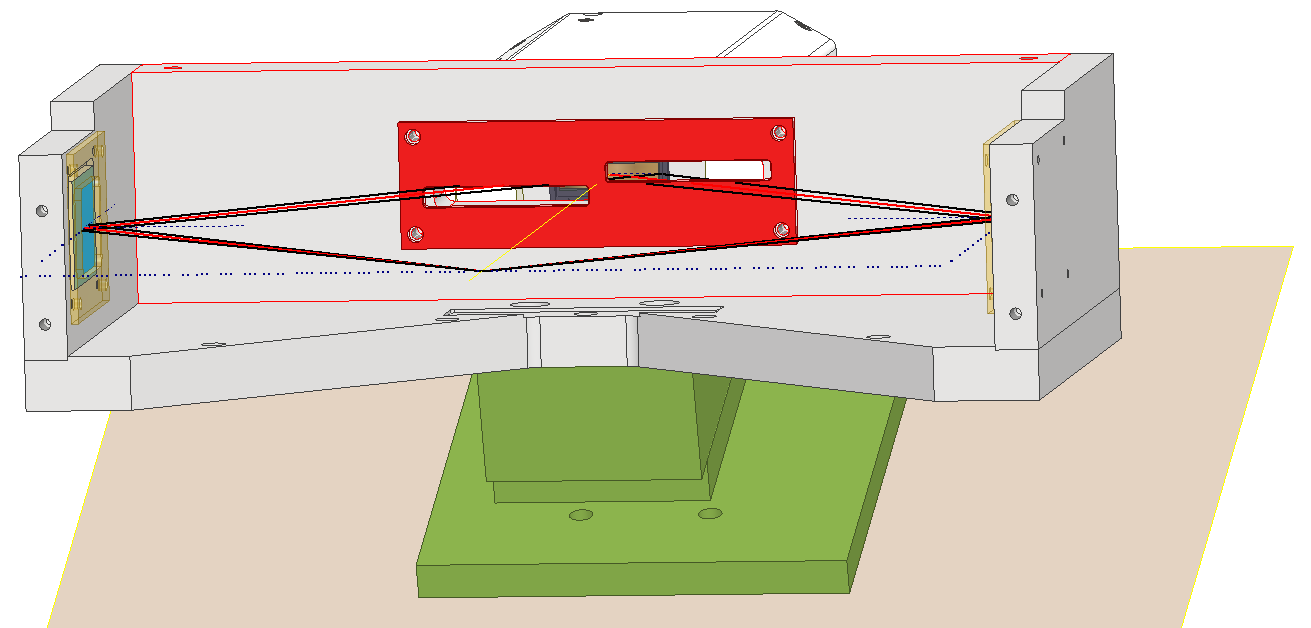
\includegraphics[width=\textwidth]{InventorPics/DUCCFilterView.PNG}
		\caption{Front view with top and inner shielding as well 
		as the pointer 
		holder hidden.}
		\label{InvDUCCPartFilter}
	\end{subfigure}
	\caption{CAD model of the DUCC. The parts are color coded, 
	whose 
	function and name are listed in table \ref{Table: DUCC 
	colors}.
	The optical posts between the foot parts are not depicted.}
	\label{InvDUCC}
\end{figure}

\begin{figure} [H]
	\centering
	\begin{subfigure}[t]{0.45\textwidth}
		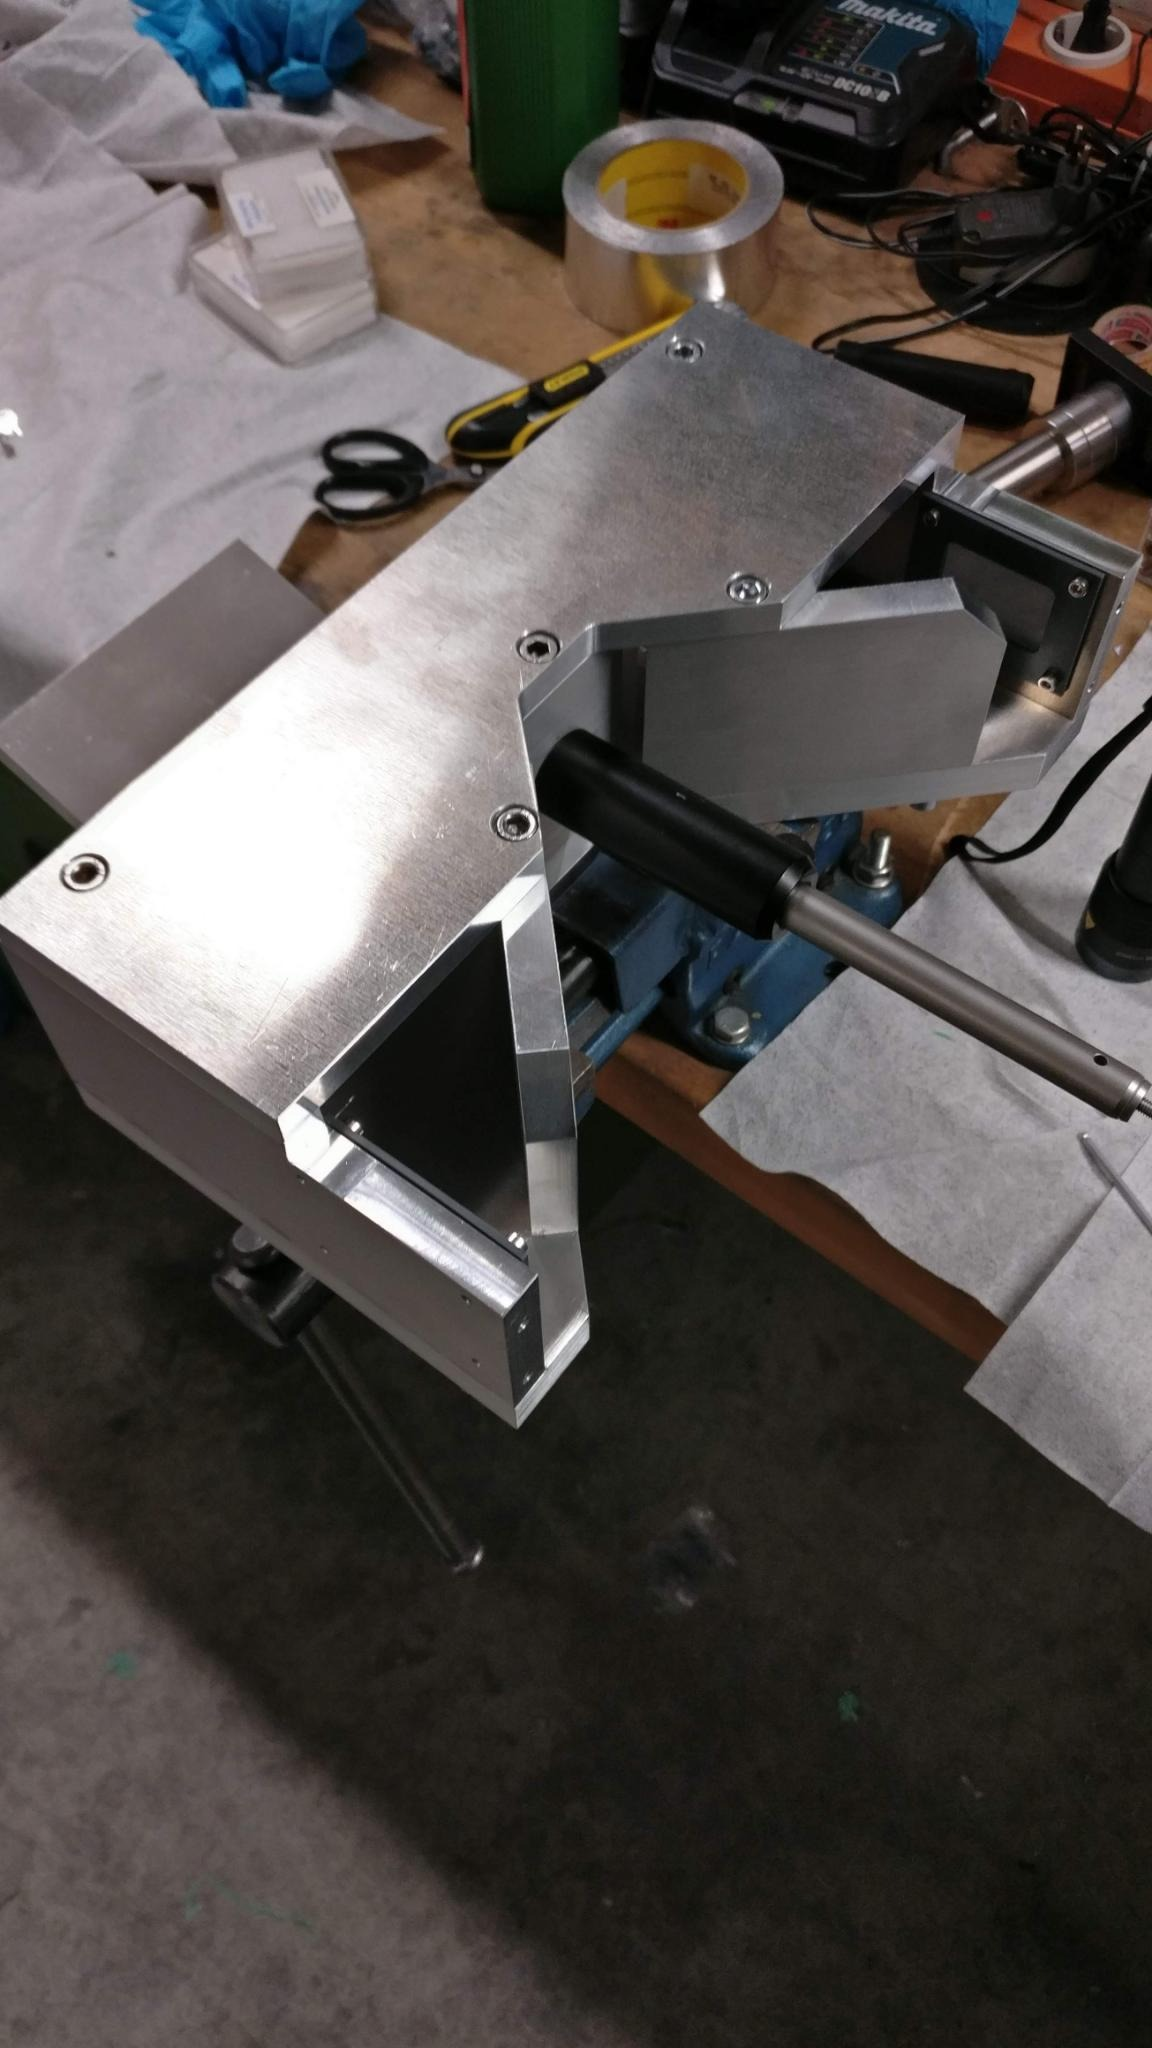
\includegraphics[width=\textwidth]{InventorPics/Real_pic_DUCC_complete.jpeg}
		\caption{Top view.}
	\end{subfigure}%
	\hfill
	\begin{subfigure}[t]{0.45\textwidth}
		\centering
		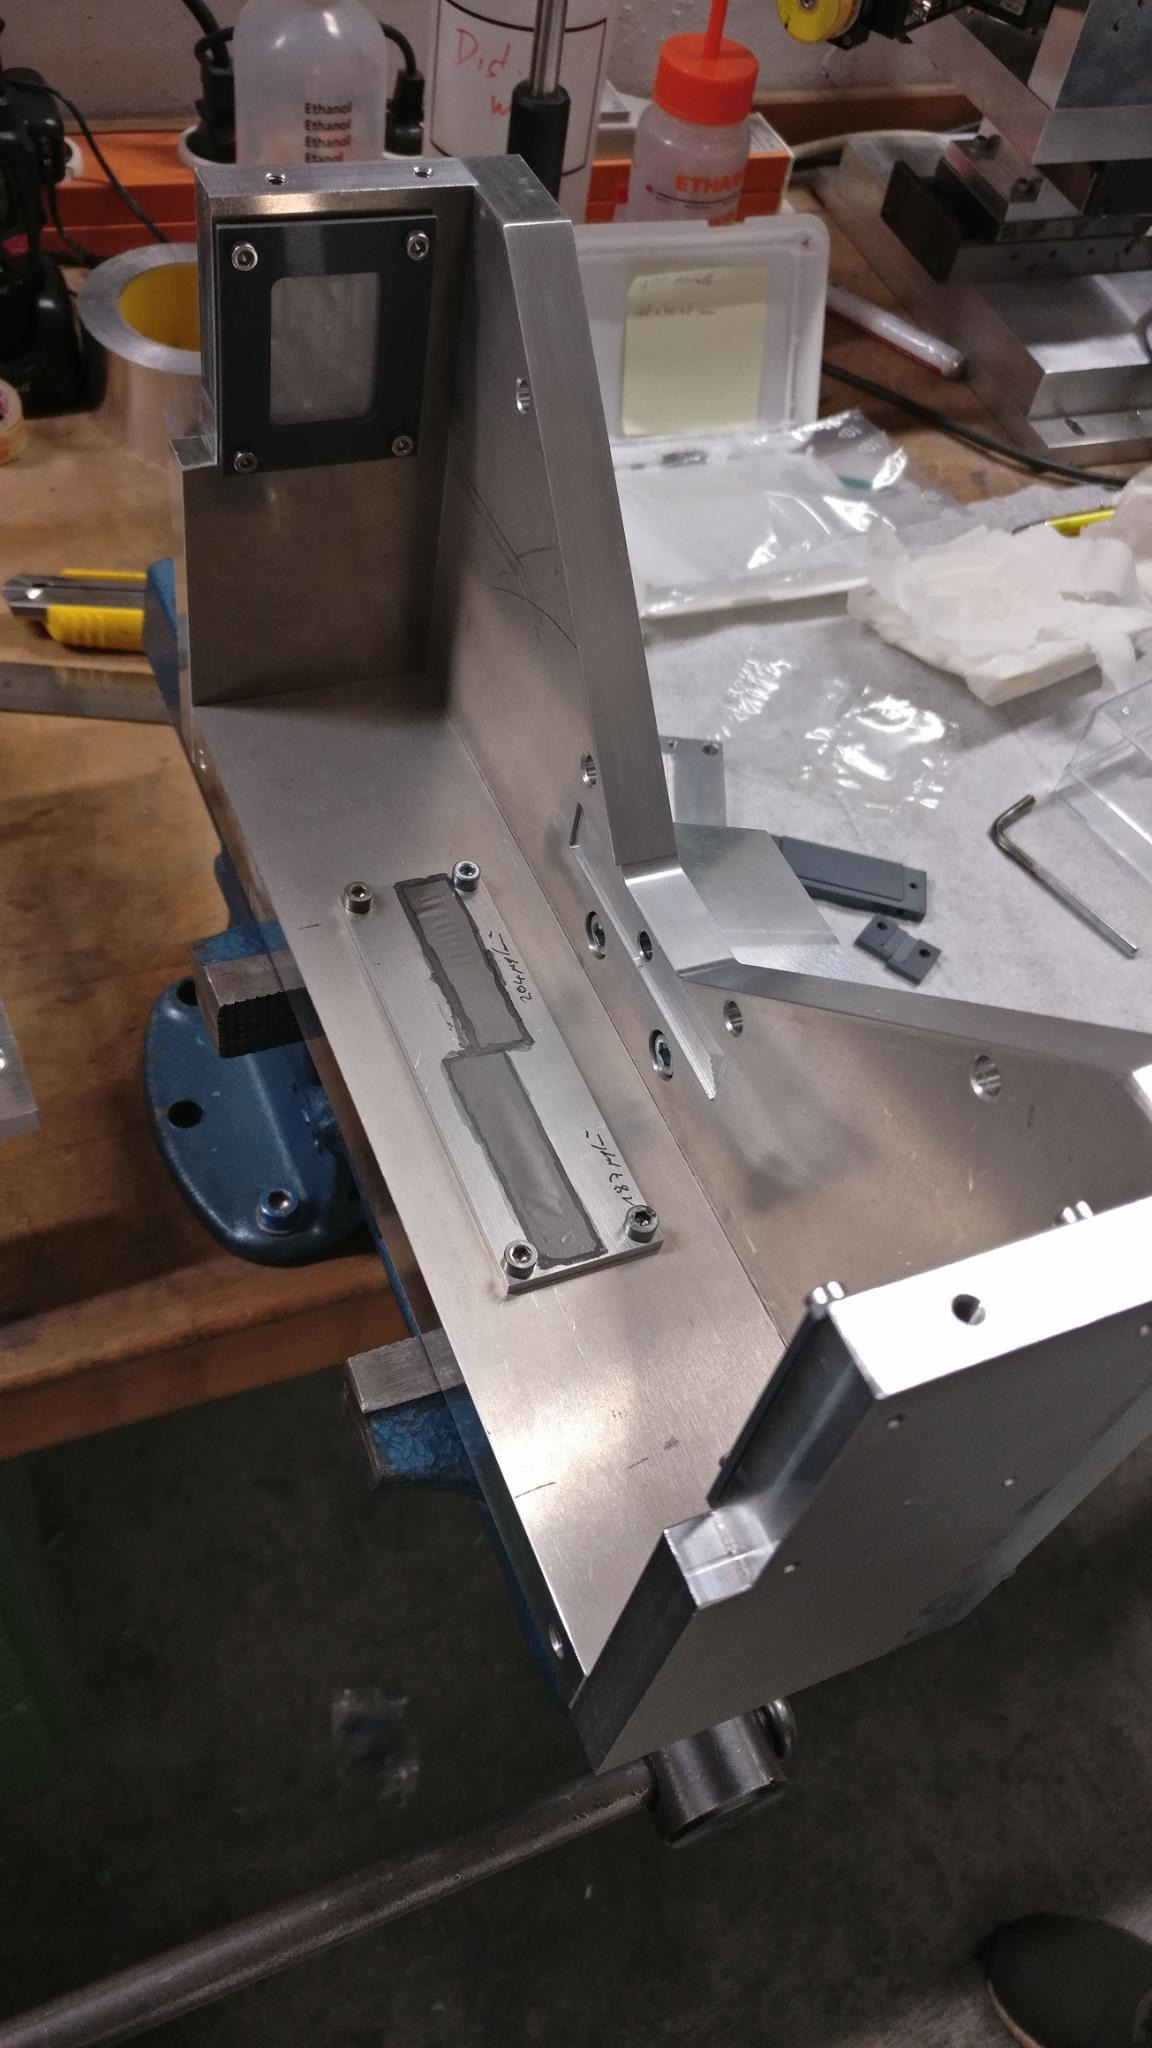
\includegraphics[width=\textwidth]{InventorPics/Real_pic_DUCC_inside.jpeg}
		\caption{Inside view.}
	\end{subfigure}\\[1ex]
	\caption{Pictures of the DUCC before the experiment without the camera.}
\end{figure}

\subsection{Focusing Spectrograph with Spatial Resolution}

In fig. \ref{InvFSSR} the FSSR-1D model is pictured with the 
parts 
color coded, presented in table \ref{Table: FSSR colors} with 
a summary of their functions and names. The shielding in this 
setup is mainly taken care of by the front plate closest to TCC. 
A 
snout, formed by three plates, adds additional shielding in 
front of the chip, as well as functioning as an aperture at the 
polychromatic crossover as described in section 
\ref{SectionTheoryFSSR}. Inside the 
snout is the carbon filter 
holder, which fulfills the same role as with the DUCC, except 
this time 
using only the $\approx\SI{900}{\micro\gram\per\cm\squared}$ 
carbon 
filter. Additionally, a blast shield is attached to the front 
plate, 
set up the same way as in the DUCC. The crystal itself was originally planned 
to be fixed 
by the 
crystal holder, designed in such a way that the reflecting 
surface does 
not come into contact with anything. In the experiment, this holder couldn't be 
used, as the mica crystal was a different one than planned, namely one that 
came in its own holder. 

\begin{table}[H]
	\centering
	\caption{Color code of the FSSR-1D model with the functions and 
		name of 
		the parts. Note that there are four optical stages which are not 
		color 
		coded. These are used in the alignment process, so are labeled in 
		fig. 
		\ref{InvFSSRAlignment}.}
	\vspace{0.05cm}
	\renewcommand{\arraystretch}{1.5}
	\centering
	\begin{tabular}{|c|c|c|} 
		\hline
		Color & Function & Name \\ [0.5ex]
		\hline\hline
		Light gray & Structural/Shielding & - \\ 
		[0.5ex]
		\hline
		Light gray (labeled) & Capturing spectra & Greateyes camera \\ 
		[0.5ex]
		\hline
		Brown & Capturing spectra & Camera chip \\ 
		[0.5ex]
		\hline
		White & Aperture at crossover/Shielding & Snout \\ 
		[0.5ex]
		\hline
		Dark gray & Securing crystal & Crystal holder \\ 
		[0.5ex]
		\hline
		Red (front of camera) & Holding carbon filter & 
		Filter holder \\ [0.5ex]
		\hline
		Dark blue & Protecting crystal & Blast shield \\ 
		[0.5ex]
		\hline
		Turquoise & Dispersion of rays & Mica crystal \\ [0.5ex]
		\hline
		Green & Support & Foot \\ 
		[0.5ex]
		\hline
		Beige & Display location of chamber floor & Breadboard floor \\ 
		[0.5ex]
		\hline
		Red & - & Central ray \\ 
		[0.5ex]
		\hline
		Black & - & Outer rays \\ [0.5ex]
		\hline
		Olive green & - & Highest energy ray \\ [0.5ex]
		\hline
	\end{tabular}
	\label{Table: FSSR colors}
\end{table}

Shown in fig. \ref{InvFSSR} are also optical stages utilized 
for the 
alignment procedure, which 
must be more exacting than that of the DUCC, owing to the 
curvature of the 
crystal and therefore the imaging and focusing properties. 
As the 
alignment is 
an involved process using additional components not pictured 
in fig. 
\ref{InvFSSR}, it is described in detail in the appendix, section 
\ref{section: 
	FSSR-1D alignment}.

The precision of the internal alignment of $\pm$\SI{0.5}{\milli\meter} is 
realized with a series of grooves, where each part attached to the main plate 
is set into a groove. The alignment process use the various optical stages 
further guarantees the desired precision.


\begin{figure} [H]
	\centering
	\begin{subfigure}[t]{0.42\textwidth}
		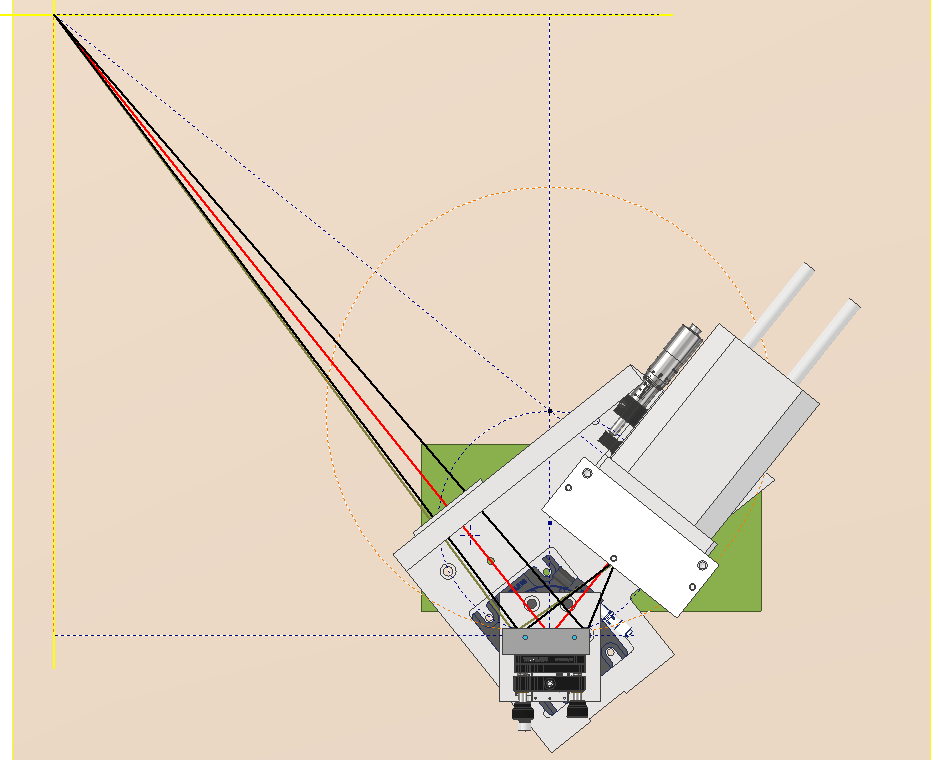
\includegraphics[width=\textwidth]{InventorPics/FSSRFullTop.PNG}
		\caption{Top view.}
		\label{InvFSSRFullTop}
	\end{subfigure}%
	\hfill
	\begin{subfigure}[t]{0.56\textwidth}
	\centering
		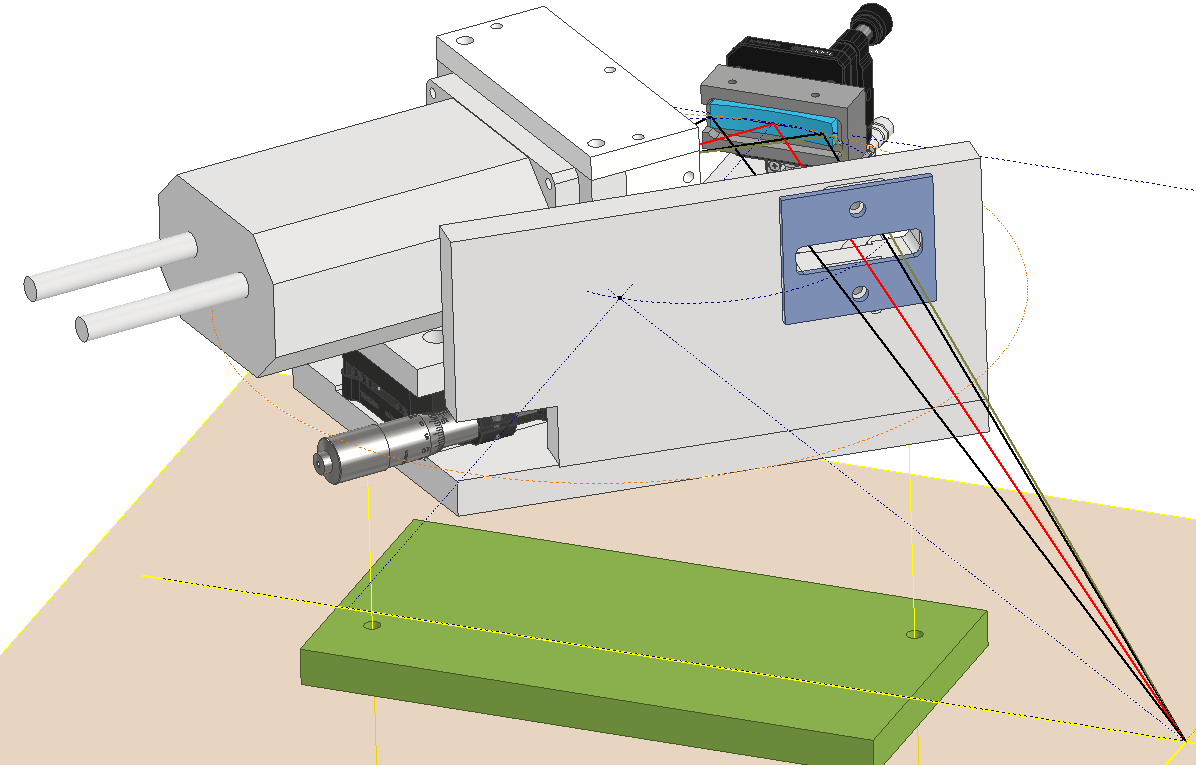
\includegraphics[width=\textwidth]{InventorPics/FSSRFullFront.PNG}
		\caption{Front view.}
		\label{InvFSSRFullFront}
	\end{subfigure}\\[1ex]
	\centering
	\begin{subfigure}[t]{0.6\textwidth}
	\centering
		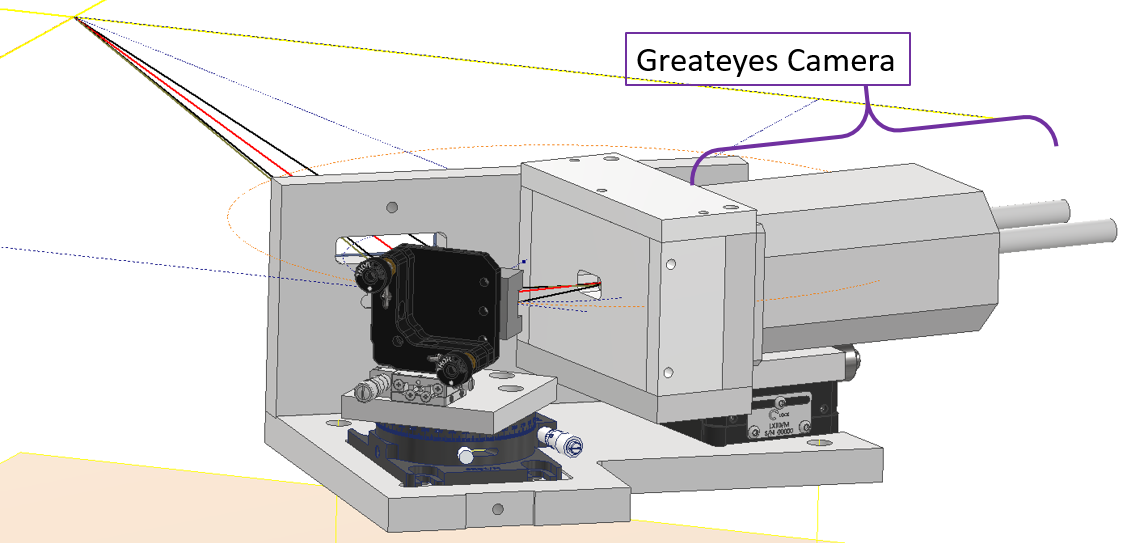
\includegraphics[width=\textwidth]{InventorPics/FSSRFullBack.PNG}
		\caption{Back view with Greateyes camera labeled.}
		\label{InvFSSRFullBack}
	\end{subfigure}%
	\begin{subfigure}[t]{0.38\textwidth}
	\centering
		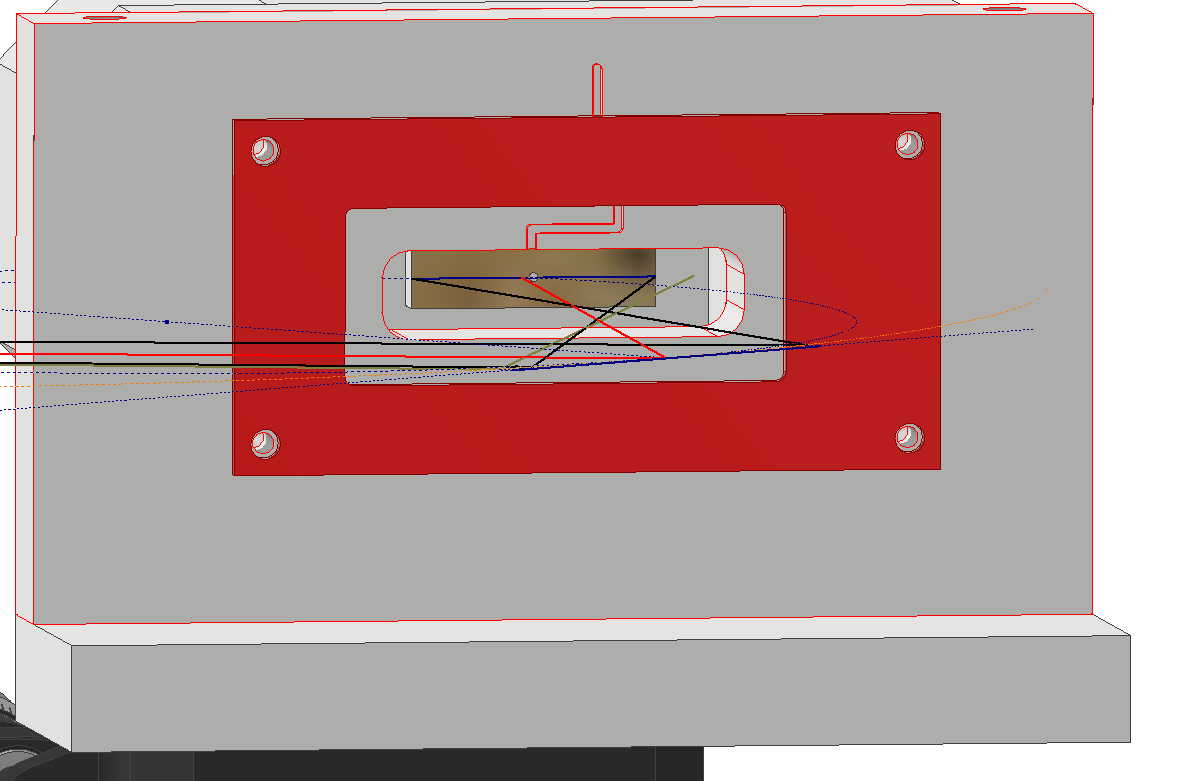
\includegraphics[width=\textwidth]{InventorPics/FSSRCameraNoSnout.PNG}
		\caption{View onto chip with snout and camera apparatus 
		hidden. 
		Venting channel is shown behind the filter holder.}
		\label{InvFSSRPartCamera}
	\end{subfigure}
	\caption{CAD model of the FSSR-1D. The parts are color coded, 
	whose 
	function and name are listed in table \ref{Table: FSSR 
	colors}. 
	Note that the optical posts between foot and bottom plate are 
	not 
	shown. The various optical stages for aligning the 
	spectrometer are 
	shown, but not color coded.}
	\label{InvFSSR}
\end{figure}

\begin{figure}[H]
	\centering
	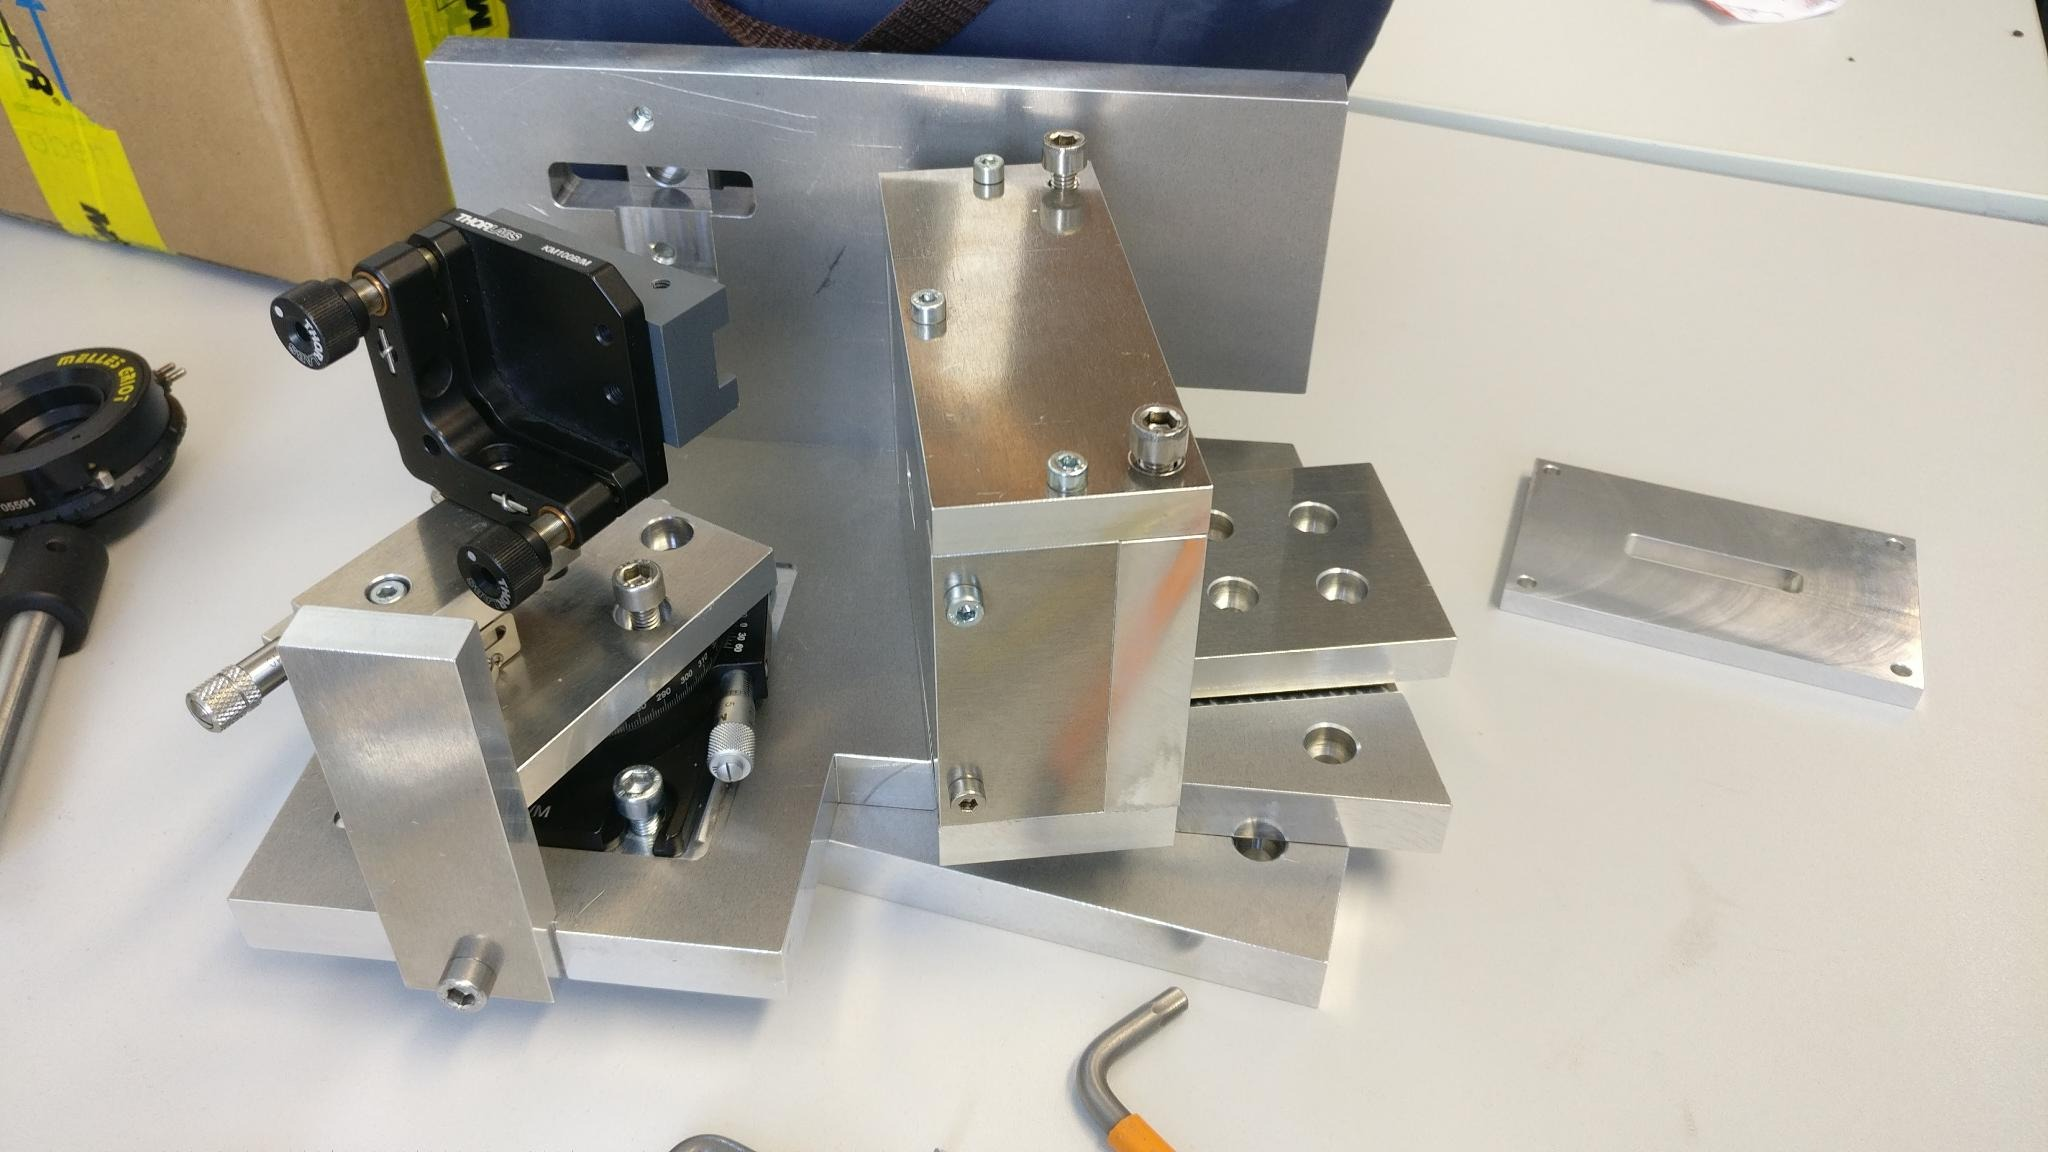
\includegraphics[width = 0.95\textwidth]{InventorPics/Real_pic_FSSR.jpeg}
	\caption{Picture of the FSSR before the experiment without the camera.}
\end{figure}




